\chapter{Preliminaries}
\label{c:preliminaries}



In this chapter we will introduce the basics of this work both to clarify notation and to introduce the reader to potentially unknown concepts and methodologies. We will start by having a look at dynamical systems that form the basis of this thesis.

\section{Dynamical Systems}  % TODO: Maybe drop completely?
	A \emph{dynamical system}~\cite{birkhoffDynamicalSystems1927} is a (physical) system that evolves over time \(t\) and is completely defined by the values of \(m\) real variables
	\begin{equation*}
		x_1, x_2, \,\cdots\!, x_m \quad\longleftrightarrow\quad \vec{x} = \begin{bmatrix} x_1 & x_2 & \cdots & x_m \end{bmatrix}^T
	\end{equation*}
	called the \emph{state} and often written in vector form (right). Given the differentiability of these values, we can also study their rate of change (often referred to as the "velocity") and the rate of change of the velocity (often referred to as the "acceleration"):
	\begin{equation*}
		\dot{\vec{x}} = \dv{\vec{x}}{t} \qquad \ddot{\vec{x}} = \dv[2]{\vec{x}}{t}
	\end{equation*}
	Describing these systems is possible using differential equations, both ordinary and partial ones. A general \(k\)-th order \ac{ode} is given by an implicit equation
	\begin{equation}
		\vec{0} = \vec{F}\big( \vec{x}, \vec{x}^{(1)}, \vec{x}^{(2)}, \,\cdots\!, \vec{x}^{(k - 1)}, \vec{x}^{(k)}; t \big),\quad \vec{x}^{(l)} \coloneqq \dv[l]{\vec{x}}{t}  \label{eq:ode}
	\end{equation}
	which establishes a connection between the state itself and its time derivatives. We call a function \( \vec{x}(t) \) a \emph{solution} of an \ac{ode} if its derivatives fulfill the given \ac{ode}~\eqref{eq:ode}. In all of the following, we assume to have explicit, autonomous, first order \acp{ode}. This is valid because we can transform every explicit higher order \ac{ode} into a system of first order \acp{ode}. Also we can introduce another "clock state" which makes our \ac{ode} autonomous.

	The solution theory for linear \acp{ode} is highly evolved and solutions exist for nearly every possible \ac{ode}. But for nonlinear \acp{ode}, we do not have such solution theories. With the exception of some rare cases, nonlinear \acp{ode} are not tractable. Hence, we often need approximations for the nonlinear case. Some well-known approaches for these approximations are \eg \emph{small angle approximation} for Sines and Cosines. In small angle approximations, we Taylor-expand \( \sin \)/\( \cos \) at \( \varphi_a = 0 \) and cut all higher order terms:
	\begin{gather*}
		\sin(\varphi) = \varphi - \underbrace{\frac{\varphi^3}{3!} + \frac{\varphi^5}{5!} + \cdots}_\text{higher order terms} \approx \varphi \\
		\cos(\varphi) = 1 - \underbrace{\frac{\varphi^2}{2!} + \frac{\varphi^4}{4!} - \frac{\varphi^6}{6!} + \cdots}_\text{higher order terms} \approx 1
	\end{gather*}
	This approach is illustrated in~\autoref{fig:smallAngleApproximation}.

	\begin{figure}
		\centering
		\begin{subfigure}[t]{0.5\linewidth}
			\centering
			\includegraphics[width = \linewidth]{figures/introduction/generated/small-angle-approximation-sin.png}
			\caption[Small angle approximation of sine]{Small angle approximation \( \sin(\varphi) \approx \varphi \) of Sine.}
		\end{subfigure}%
		~
		\begin{subfigure}[t]{0.5\linewidth}
			\centering
			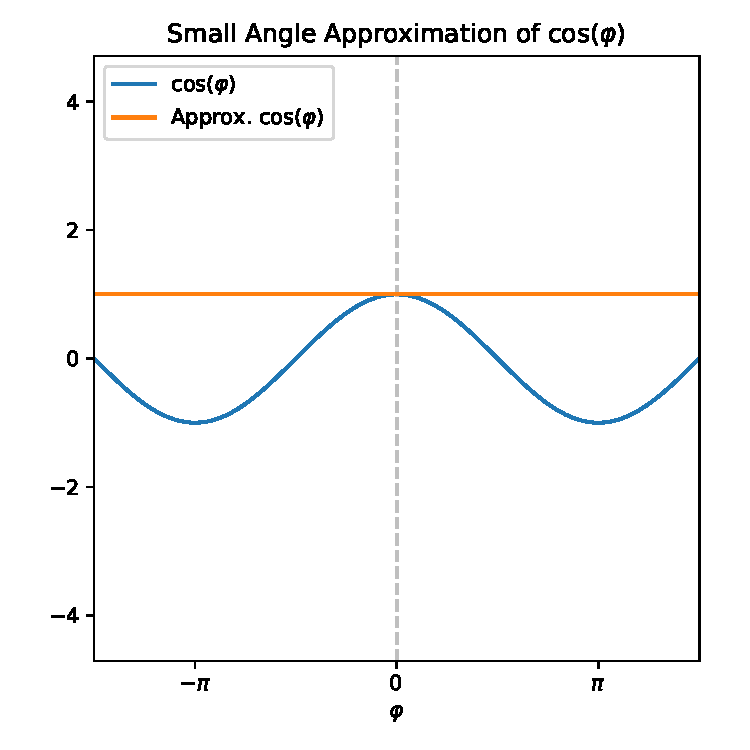
\includegraphics[width = \linewidth]{figures/introduction/generated/small-angle-approximation-cos.png}
			\caption[Small angle approximation of cosine]{Small angle approximation \( \cos(\varphi) \approx 1 \) of Cosine.}
		\end{subfigure}
		\caption[Small angle approximation of sine and cosine]{Visualization of the small angle approximation (given in orange) of the basic trigonometric functions Sine and Cosine (given in blue). It is clear that the approximation is only valid in a small region around zero (\( \varphi \approx 0 \)).}
		\label{fig:smallAngleApproximation}
	\end{figure}

	We now look at two examples of dynamical systems, firstly at a linear one and secondly at a nonlinear one.

	\paragraph{Harmonic Oscillator}
		\label{subsec:harmonicOscillator}

		\begin{figure}
			\centering
			\tikzHarmonicOscillator
			\caption[Illustration of a simple harmonic oscillator]{Illustration of a simple harmonic oscillator with mass \(m\), spring stiffness \(k\) and position \(x\) that is not affected by any external force like gravity. The mass is in equilibrium if \( x = 0 \).}
			\label{fig:simpleHarmonicOscillator}
		\end{figure}

		The \emph{simple harmonic oscillator} describes the dynamical system of a mass \(m\) that is attached to a spring that is following Hooke's Law with stiffness \(k\) (see~\autoref{fig:simpleHarmonicOscillator}). This harmonic oscillator is described by the \ac{ode}
		\begin{equation}
			m\ddot{x} = -kx \quad\iff\quad \ddot{x} = -\frac{k}{m} x  \label{eq:harmonicOscillator}
		\end{equation}
		where \(x\) and \(\ddot{x}\) are the position and acceleration of the mass, respectively. Note that if \( x = 0 \), the mass is in equilibrium and no force is acting on it.

		By using basic results in the solution theory of linear \acp{ode}, we see that the general solution is given as
		\begin{equation*}
			x(t) = A \cos\Big(t \sqrt{k / m} + \varphi\Big)
		\end{equation*}
		with the amplitude \(A\) and the phase \(\varphi\) (see~\autoref{app:harmonicOscillatorSolution} for the derivation of the solution). As neither gravity nor damping or other external forces are involved in the dynamical system, the motion continues forever with a non-changing amplitude.
	% end

	\paragraph{Inverse Pendulum}
		\label{subsec:simplePendulum}

		\begin{figure}
			\centering
			\tikzSimplePendulum
			\caption[Illustration of an inverse pendulum]{Illustration of an inverse pendulum with mass \(m\) and displacement \(\varphi\) that is only affected by gravity and no other external force. The mass is in equilibrium for both \( \varphi = 0 \) and \( \varphi = \pi \), where the former is an unstable equilibrium.}
			\label{fig:simplePendulum}
		\end{figure}

		The \emph{inverse pendulum} describes the dynamical system of a mass \(m\) that is attached to a rigid pole of length \(L\) which can freely swing around a suspension point (see~\autoref{fig:simplePendulum}). The pendulum stands upright if \( \varphi = 0 \) and its equation of motion is described by the \ac{ode}
		\begin{equation*}
			\ddot{\varphi} = \frac{g}{L} \sin(\varphi)
		\end{equation*}
		where \(g\), \(L\), \(\varphi\) and \(\ddot{\varphi}\) describe the gravity acceleration, pole length, displacement and acceleration of the mass, respectively. Note that if \( \varphi = 0 \), the mass is in an unstable equilibrium and no force is acting on it.

		In comparison to the harmonic oscillator (\autoref{subsec:harmonicOscillator}), this differential equation is nonlinear. And, even for the case with unit gravity acceleration \( g = 1 \) and unit pole length \( L = 1\), where the \ac{ode} looks really simple
		\begin{equation}
			\ddot{\varphi} = \sin(\varphi)  \label{eq:inversePendulum}
		\end{equation}
		it is not tractable analytically (\ie there exists no solution in closed form).

		Still, we can apply the small angle approximation introduced before (in this case, \( \sin(\varphi) \approx \varphi \)) which yields the simple \ac{ode}
		\begin{equation}
			\ddot{\varphi} \approx \varphi  \label{eq:linearizedInversePendulum}
		\end{equation}
		solved by
		\begin{equation*}
			\varphi(t) = \frac{1}{2} e^{-t} \big(\varphi_0 + e^{2t} \varphi_0 - \dot{\varphi}_0 + e^{2t} \dot{\varphi}_0\big)
		\end{equation*}
		where \(\varphi_0\) and \(\dot{\varphi}_0\) are the initial displacement and velocity, respectively.

		However, this small angle approximation can only forecast small displacements \( \varphi \ll \pi/2 \). And, as the equilibrium at \( \varphi = 0 \) is unstable, the approximation becomes worse as time goes by because the pendulum falls down. This behavior is shown in~\autoref{fig:inversePendulumApprox}.

		\begin{figure}
			\centering
			\begin{subfigure}[t]{0.5\linewidth}
				\centering
				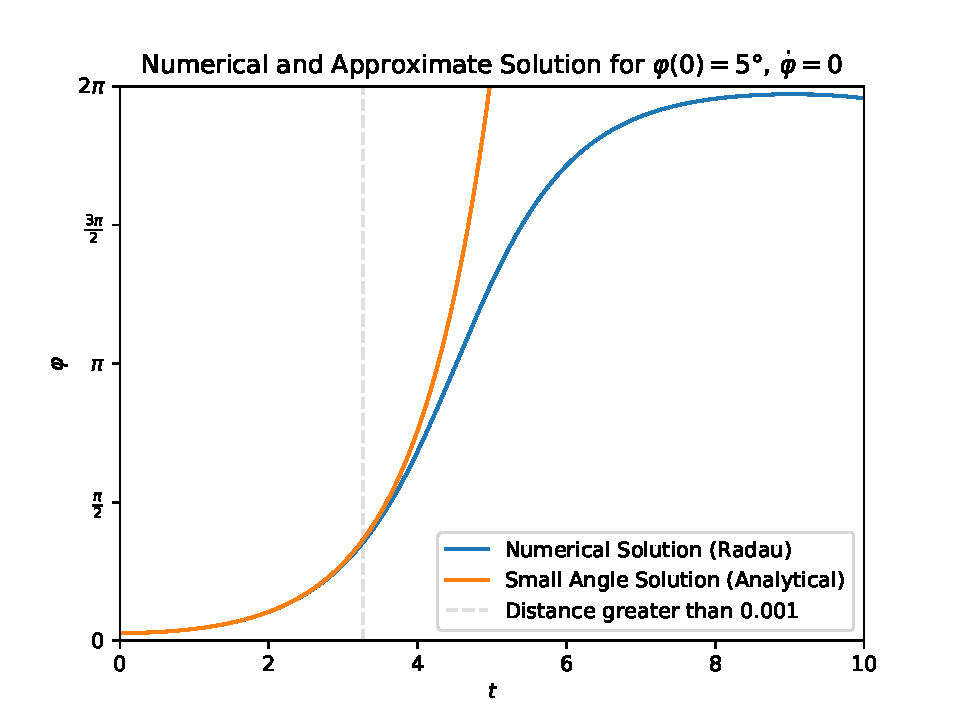
\includegraphics[width = \linewidth]{figures/introduction/generated/pendulum-motion-solutions}
				\caption[Trajectories of the small angle approximate solution of the inverse pendulum and a numerical solution]{Trajectories of two solution strategies to the inverse pendulum, where the blue is a numerical solution of the actual motion of equation (solved using the Radau~IIA method~\cite[p.~72]{guglielmiImplementingRadauIIA2001}) and the orange one is the analytically computed solution linearized \ac{ode}. The latter is linearized using small angle approximation. The dashed gray vertical line shows when the distance tolerance of \( \varepsilon = 10^{-3} \) is exceeded.}
			\end{subfigure}%
			~
			\begin{subfigure}[t]{0.5\linewidth}
				\centering
				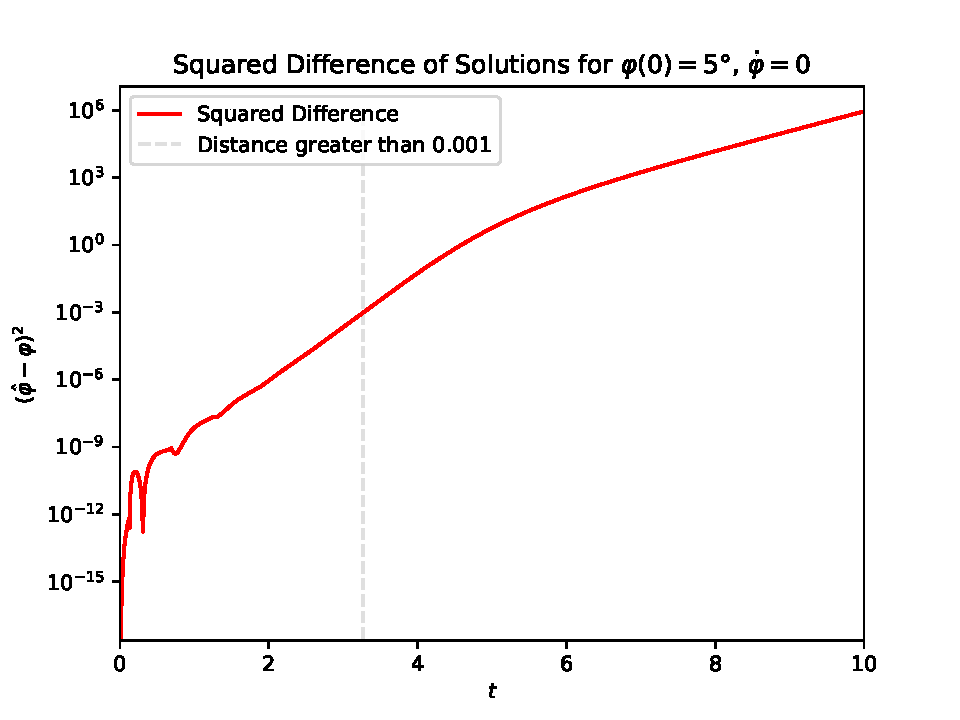
\includegraphics[width = \linewidth]{figures/introduction/generated/pendulum-motion-difference}
				\caption[Difference between the small angle approximate solution of the inverse pendulum and a numerical solution]{Differences between the small angle approximation and the numerical solution of the \ac{ode}. The dashed gray vertical line shows when the distance tolerance of \( \varepsilon = 10^{-3} \) is exceeded.}
			\end{subfigure}
			\caption[Comparison of the small angle approximate solution of the inverse pendulum and a numerical solution]{Comparison of a numerical solution to the \ac{ode} of the inverse pendulum given in~\eqref{eq:inversePendulum} and the analytical solution of the linearized \ac{ode} given in~\eqref{eq:linearizedInversePendulum}. A tolerance value of \( \varepsilon = 10^{-3} \) is used to show when both solutions diverge from each other.}
			\label{fig:inversePendulumApprox}
		\end{figure}
	% end

	\subsection{Discrete-Time Dynamical Systems}
		In comparison to continuous-time dynamical systems described by \acp{ode}, discrete-time systems are described by a \emph{dynamics function} \( \vec{F} : \R^n \to \R^n \) advancing all states forward in time:
		\begin{equation*}
			\vec{x}_{t + 1} = \vec{F}(\vec{x}_t)
		\end{equation*}
		But we should note that, while seeming more restrictive, discrete-time dynamical systems are more general~\cite{bruntonKoopmanInvariantSubspaces2016} than continuous-time systems as we can discretize every continuous-time system
		\begin{equation*}
			\dot{\vec{x}} = \vec{f}(\vec{x})
		\end{equation*}
		as a discrete-time dynamical system
		\begin{equation*}
			\vec{x}_{t + 1} = \vec{F}(\vec{x}_t)
		\end{equation*}
		using the state dynamics function
		\begin{equation*}
			\vec{F}\big(\vec{x}(t_0)\big) = \vec{x}(t_0 + \Delta_t) = \vec{x}(t_0) + \int_{t_0}^{t_0 + \Delta_t} \! \vec{f}\big(\vec{x}(\tau)\big) \dd{\tau}
		\end{equation*}
		where \( \Delta_t \) is called the \emph{discretization interval} and \( \vec{x}_k = \vec{x}(k \Delta_t) \).
	% end
% end

\section{Koopman Theory of Dynamical Systems}
	Our first contribution is based on the need of a linearization technique that generalizes globally. We have seen this need in the previous chapter when looking at simple nonlinear systems and small angle approximations. This brings us directly to Koopman theory, original introduced by B.~Koopman in 1931~\cite{koopmanHamiltonianSystemsTransformation1931} in the context of Hamiltonian systems and transformations in Hilbert spaces. Considering a nonlinear discrete-time dynamical system
	\begin{equation*}
		\vec{x}_{t + 1} = \vec{F}(\vec{x}_t),\quad \vec{F} : \R^k \to \R^k
	\end{equation*}
	and observations \( \vec{h} : \R^p \to \R^p \) of this system, \ie \( \vec{y}_t \coloneqq \vec{h}(\vec{x}_t) \), the infinite-dimensional \emph{Koopman operator} \(\mathcal{K}\) advances all of the measurements forward in time. This relation can also be expressed as the composition
	\begin{equation*}
		\mathcal{K} \, \vec{h} \coloneqq \vec{h} \circ \vec{F} \qquad\iff\qquad \mathcal{K} \, \vec{h}(\vec{x}_t) = \vec{h}\big( \vec{F}(\vec{x}_t) \big) = \vec{h}(\vec{x}_{t + 1})
	\end{equation*}
	and can be visualized as a transition diagram between the states (see~\autoref{fig:koopman}). This relation is true for every possible measurement function \( \vec{h} \) at any point of the system space \( \R^k \)~\cite{bruntonKoopmanInvariantSubspaces2016}. All possible measurement functions \( \vec{h} \) span an infinite-dimensional Hilbert space \( \mathcal{H} \). A finite set of measurements \( \vec{h}_1, \vec{h}_2, \cdots, \vec{h}_p \) that span an invariant subspace \( \hat{\mathcal{H}} \subset \mathcal{H} \) can be considered as a basis of that subspace. That is, applying the Koopman operator to a linear combination of these functions keeps them in the subspace:
	\begin{align*}
		\vec{h} &= \alpha_1 \vec{h}_1 + \alpha_2 \vec{h}_2 + \cdots + \alpha_p \vec{g}_p \\
		\mathcal{K} \, \vec{h} &= \beta_1 \vec{h}_1 + \beta_2 \vec{h}_2 + \cdots + \beta_p \vec{h}_p
	\end{align*}
	If that is possible, we can restrict the Koopman operator onto \( \hat{\mathcal{H}} \). Functions that both span the subspace \(\hat{\mathcal{H}}\) and do only scale when applying the Koopman operator, \ie \( \mathcal{K} \, \vec{\varphi} = \lambda \vec{\varphi} \) are called \emph{eigenfunctions} of the Koopman operator. Finding these eigenfunctions is extremely desirable as it allows us to get a finite Koopman operator matrix \( \mat{K} \) globally linearizing the dynamical system \( \vec{F} \). However, for this thesis, we do not seek the eigenfunctions directly but an approximation of the \emph{inverse} observation function to forecast the dynamical system.

	\begin{figure}
		\centering
		\tikzKoopmanOperator
		\caption[State transition model of a Koopman dynamical system]{Illustration of the transition diagram imposed by applying the Koopman operator \( \mathcal{K} \) to system dynamics \( \vec{F} \). The observation function \( \vec{h} \) is forwarded in time linearly by the Koopman operator, while the states \(\vec{x}\) are forwarded nonlinearly. The dashed lines and \( \vec{h}^{-1} \) indicate that we want to recover the original state from the linear system. \\ Adopted from~\cite{bruntonKoopmanInvariantSubspaces2016}.}
		\label{fig:koopman}
	\end{figure}
% end

\section{The Expectation-Maximization Algorithm}
	\label{sec:em}

	The \ac{em} algorithm, first introduced by Ceppellini et al. in 1955~\cite{ceppelliniEstimationGeneFrequencies1955} and popularized by Dempster et al. in 1977~\cite{dempsterMaximumLikelihoodIncomplete1977a} can be used for tackling the following problem: Assuming some model with latent (hidden) states \(\vec{x}\), observations \(\vec{y}\) and model parameters \(\vec{\theta}\), we want to maximize the likelihood \( p(\vec{y} \given \vec{\theta}) \) \ac{wrt} the latent states \(\vec{x}\) and the parameters \(\vec{\theta}\). However, the marginal distribution
	\begin{align*}
		p(\vec{y} \given \vec{\theta}) = \int\! p(\vec{x}, \vec{y} \given \vec{\theta}) \dd{\vec{x}}
	\end{align*}
	is generally intractable. As usual on maximum likelihood approaches, it is useful not to maximize the likelihood directly, but to maximize the log-likelihood
	\begin{align*}
		\mathcal{L}(\vec{\theta}) \coloneqq \log p(\vec{y} \given \vec{\theta}) = \log \int\! p(\vec{x}, \vec{y} \given \vec{\theta}) \dd{\vec{x}}
	\end{align*}
	instead. This yields the same maximum as the logarithm is strictly increasing. By introducing an auxiliary probability distribution \( q(\vec{x} \given \vec{y}) \) over the latent variables, we can rewrite the marginal and find a lower bound on \(\mathcal{L}\) by using Jensen's inequality~\cite{jensenFonctionsConvexesInegalites1906}:
	\begin{align}
		\mathcal{L}(\vec{\theta})
			&= \log \int\! p(\vec{x}, \vec{y} \given \vec{\theta}) \dd{\vec{x}}  \nonumber \\
			&= \log \int\! q(\vec{x} \given \vec{y}) \frac{p(\vec{x}, \vec{y} \given \vec{\theta})}{q(\vec{x} \given \vec{y})} \dd{\vec{x}}  \nonumber \\
			&\geq \int\! q(\vec{x} \given \vec{y}) \log \frac{p(\vec{x}, \vec{y} \given \vec{\theta})}{q(\vec{x} \given \vec{y})} \dd{\vec{x}}  \nonumber \\
			&= \int\! q(\vec{x} \given \vec{y}) \log p(\vec{x}, \vec{y} \given \vec{\theta}) \dd{\vec{x}} - \int\! q(\vec{x} \given \vec{y}) \log q(\vec{x} \given \vec{y}) \dd{\vec{x}} \eqqcolon \mathcal{L}_\mathrm{EM}[q, \vec{\theta}]  \label{eq:emLowerBound}
	\end{align}
	This draws a lower bound \( \mathcal{L}_\mathrm{EM}[q, \vec{\theta}] \) on the log-likelihood \( \mathcal{L}(\vec{\theta}) \) we can maximize instead, maximizing the log-likelihood simultaneously. Note that this lower bound is in fact a functional of the distribution \( q(\vec{x} \given \vec{y}) \).

	The \ac{em} algorithm now iteratively maximizes the lower bound and thus indirectly maximizes the original objective, the likelihood \( p(\vec{y} \given \vec{\theta}) \). The E and M step are as follows:
	\begin{description}
		\item[E-Step] Infers the auxiliary distribution \( q(\vec{x} \given \vec{y}) \) using the current estimations of the parameters \( \vec{\theta} \) by maximizing the lower bound \ac{wrt} the auxiliary distribution.
		\item[M-Step] Infers the parameters \(\vec{\theta}\) using the current auxiliary distribution by maximizing the lower bound \ac{wrt} the parameters.
	\end{description}
	Expressed in equations with the index \( \cdot^{(n)} \) to denote the values of the \(n\)-th iteration, we get the procedure which will be repeated until convergence:
	\begin{description}
		\item[E-Step] \eqparbox[r]{emSteps}{\(\displaystyle q^{(n + 1)} \)} \(\displaystyle = \arg\max_{q}\, \mathcal{L}_\mathrm{EM}\big[ q, \vec{\theta}^{(n)} \big] \)
		\item[M-Step] \eqparbox[r]{emSteps}{\(\displaystyle \vec{\theta}^{(n + 1)} \)} \(\displaystyle = \arg\max_{\vec{\theta}}\, \mathcal{L}_\mathrm{EM}\big[ q^{(n + 1)}, \vec{\theta} \big] \)
	\end{description}
	Additionally, the E-step has the constraint that \(q(\vec{x} \given \vec{y})\) really is a probability distribution, so it must integrate to one:
	\begin{align*}
		\int\! q(\vec{x} \given \vec{y}) \dd{\vec{x}} = 1
	\end{align*}
	We can incorporate this into the maximization, \eg using Lagrange multipliers. Using a bit of variational calculus, it can be shown~\cite{bealVariationalAlgorithmsApproximate2003a} that the maximization is gained by choosing the auxiliary distribution \(q(\vec{x} \given \vec{y})\) to be the same as the distribution \( p(\vec{x} \given \vec{y}, \vec{\theta}) \). That is, we set \( q^{(n + 1)}(\vec{x} \given \vec{y}) = p\big(\vec{x} \biggiven \vec{y}, \vec{\theta}^{(n)}\big) \) while holding the parameters \(\vec{\theta}\) fixed. This maximization turns the lower bound into an equality with the actual likelihood.

	For the M-step, we keep the auxiliary distribution fixed and maximize the lower bound \ac{wrt} the parameters~\(\vec{\theta}\). As this involves taking the derivative of \(\mathcal{L}_\mathrm{EM}\) \ac{wrt} \(\vec{\theta}\), we can safely omit the right hand side of the lower bound as it does not depend on \(\vec{\theta}\). Hence, we get the M-step as:
	\begin{align*}
		\vec{\theta}^{(n + 1)}
			&= \arg\max_{\vec{\theta}}\, \mathcal{L}_\mathrm{EM}\big[ q^{(n)}, \vec{\theta} \big] \\
			&= \arg\max_{\vec{\theta}} \int\! q^{(n)}(\vec{x} \given \vec{y}) \log p(\vec{x}, \vec{y} \given \vec{\theta}) \dd{\vec{x}} \\
			&= \arg\max_{\vec{\theta}} \int\! p\big(\vec{x} \biggiven \vec{y}, \vec{\theta}^{(n)}\big) \log p(\vec{x}, \vec{y} \given \vec{\theta}) \dd{\vec{x}} \\
			&= \arg\max_{\vec{\theta}}\, \E_{p(\vec{x} \given \vec{y}, \vec{\theta}^{(n)})}[\log p(\vec{x}, \vec{y} \given \vec{\theta})]
	\end{align*}
	The quantity to optimize, \( Q(\vec{\theta}) \coloneqq \E[\log p(\vec{x}, \vec{y} \given \vec{\theta})] \), is also called the \emph{expected complete log-likelihood} as it involves both the observables and the latent variables.

	As shown in~\cite{bealVariationalAlgorithmsApproximate2003a}, the lower bound turns into an equality after the E-step. Hence, we are guaranteed to always rise the log-likelihood after each \ac{em} iteration if we do not already have the optimal auxiliary distribution and parameters. If this would be the case, both the E- and the M-step would not change anything, so our log-likelihood is monotonically increasing. Also, we might not want to calculate the whole distribution in the E-step, but we might want to restrict our computations to sufficient statistics that cover our whole distribution. For the rest of this thesis, we know our distribution \( p(\vec{x} \given \vec{y}, \vec{\theta}) \) is Gaussian, so we can assume the auxiliary distribution to be Gaussian too, given that we set them equal. Hence, we only need to calculate the mean and correlation or covariance of each variable to cover the whole distribution and to be able to proceed. This will turn out to be really useful later on.
% end

\section{Variational Autoencoders and the Evidence Lower Bound}
	Variational autoencoders have been first introduced in the context of the \ac{aevb} algorithm by Kingma and Welling in 2014~\cite{kingmaAutoEncodingVariationalBayes2014}. They tackle inference and learning in probabilistic models with latent variables, similar to the \ac{em} algorithm. To keep the notation analogous to the derivation of the \ac{em} algorithm, we deviate from~\cite{kingmaAutoEncodingVariationalBayes2014} in terms that we keep \(\vec{x}\) as our latent variables and \(\vec{y}\) as the observables.

	To perform inference, we want to maximize the (log-)\,likelihood
	\begin{align*}
		\mathcal{L}(\vec{\theta}) \coloneqq \log p_{\vec{\theta}}(\vec{y}) = \log \int\! p_{\vec{\theta}}(\vec{x}, \vec{y}) \dd{\vec{x}}
	\end{align*}
	by maximizing the \ac{elbo} \( \mathcal{L}_\mathrm{ELBO} \) which we can find by using Jensen's inequality~\cite{jensenFonctionsConvexesInegalites1906}:
	\begin{align}
		\mathcal{L}(\vec{\theta})
			&= \log \int\! p_{\vec{\theta}}(\vec{x}, \vec{y}) \dd{\vec{x}}  \nonumber \\
			&= \log \int\! q(\vec{x} \given \vec{y}, \vec{\phi}) \frac{p_{\vec{\theta}}(\vec{x}, \vec{y})}{q_{\vec{\phi}}(\vec{x} \given \vec{y})} \dd{\vec{x}}  \nonumber \\
			&\geq \int\! q_{\vec{\phi}}(\vec{x} \given \vec{y}) \log \frac{p_{\vec{\theta}}(\vec{x}, \vec{y})}{q_{\vec{\phi}}(\vec{x} \given \vec{y})} \dd{\vec{x}}  \nonumber \\
			&= \int\! q(\vec{x} \given \vec{y}, \vec{\phi}) \log \frac{p_{\vec{\theta}}(\vec{y} \given \vec{x}) p_{\vec{\theta}}(\vec{x})}{q_{\vec{\phi}}(\vec{x} \given \vec{y})} \dd{\vec{x}}  \nonumber \\
			&= \int\! q_{\vec{\phi}}(\vec{x} \given \vec{y}) \frac{p_{\vec{\theta}}(\vec{x})}{q_{\vec{\phi}}(\vec{x} \given \vec{y})} \dd{\vec{x}} + \int\! q_{\vec{\phi}}(\vec{x} \given \vec{y}) p_{\vec{\theta}}(\vec{y} \given \vec{x}) \dd{\vec{x}}  \nonumber \\
			&= -\KL{q_{\vec{\phi}}(\vec{x} \given \vec{y})}{p_{\vec{\theta}}(\vec{x})} + \E_{q_{\vec{\phi}}(\vec{x} \given \vec{y})}[p_{\vec{\theta}}(\vec{y} \given \vec{x})] \eqqcolon \mathcal{L}_\mathrm{ELBO}(\vec{\theta}, \vec{\psi})  \label{eq:elbo}
	\end{align}
	Note that we have introduced an auxiliary parametric distribution \( q_{\vec{\phi}}(\vec{x} \given \vec{y}) \) which originally leads to the first integral to be an expectation and makes the application of Jensen's inequality possible. We now maximize the \ac{elbo}~\eqref{eq:elbo} \ac{wrt} the variational and generative parameters \(\vec{\phi}\) and \(\vec{\theta}\) respectively using the \emph{reparametrization trick}~\cite{kingmaAutoEncodingVariationalBayes2014}.

	Shifting to \acp{vae}, we now represent the auxiliary distribution \( q_{\vec{\phi}}(\vec{x} \given \vec{y}) \) using a neural network with some prior \( p_{\vec{\theta}}(\vec{x}) \), e.g. a standard Gaussian \( p_{\vec{\theta}}(\vec{x}) = \normal(\vec{0}, \mat{I}) \) to keep the latents "close to the center", enforced by the \ac{kl} divergences in the \ac{elbo}. For a Gaussian latent distribution, the neural network, called the \emph{amortization network}, produces the mean and the diagonal covariance of \( q \). A second neural network is used for decoding the latent dimension, representing the decoding distribution \( p_{\vec{\theta}}(\vec{y} \given \vec{x}) \). If we assume a Gaussian decoding distribution with constant variance, the right side of the \ac{elbo}~\eqref{eq:elbo} just becomes the squared error between the decoding mean and the input \(\vec{y}\). Such a network architecture is illustrated in~\autoref{fig:vae}.

	\begin{figure}
		\centering
		\tikzVariationalAutoEncoder
		\caption[Illustration of a variational auto-encoder]{Illustration of a Variational Auto-Encoder with the amortization network on the left and the decoder network on the right. Notice that the green neurons in the middle are not "real", deterministic, neurons, but represent the sampling section of the \ac{vae} where the reparametrization takes place. The input and output size (on the left and right, respectively) are the same as we want to reconstruct our original data from the smaller latent state in the middle. Also the "latent neurons" are smaller than the in- and output neurons to enforce an encoding into a lower dimension.}
		\label{fig:vae}
	\end{figure}

	\subsection{Connection between EM and VAEs}
		As we have seen, the log-likelihood \( \mathcal{L}(\vec{\theta}) \) gives rise to a lower bound \( \mathcal{L}_\mathrm{EM} \)~\eqref{eq:emLowerBound} and the \ac{elbo} \( \mathcal{L}_\mathrm{ELBO} \)~\eqref{eq:elbo}:
		\begin{align*}
			\mathcal{L}_\mathrm{EM}[q, \vec{\theta}] &= \int\! q(\vec{x} \given \vec{y}) \log p(\vec{x}, \vec{y} \given \vec{\theta}) \dd{\vec{x}} - \int\! q(\vec{x} \given \vec{y}) \log q(\vec{x} \given \vec{y}) \dd{\vec{x}} \\
			\mathcal{L}_\mathrm{ELBO}(\vec{\theta}, \vec{\psi}) &= -\KL{q_{\vec{\phi}}(\vec{x} \given \vec{y})}{p_{\vec{\theta}}(\vec{x})} + \E_{q_{\vec{\phi}}(\vec{x} \given \vec{y})}[p_{\vec{\theta}}(\vec{y} \given \vec{x})]
		\end{align*}
		We saw that the two concepts are similar to each other, but the maximization procedure differs in the following way:
		\begin{itemize}
			\item In the \ac{em} algorithm, we separately maximize the components of the lower bound, firstly finding the next auxiliary distribution \(q\) and then maximizing the lower bound \ac{wrt} the parameters.
			\item In \acp{vae}, we use an amortization network to model the auxiliary distribution \(q\) in a parameterized way. Then we maximize the lower bound \ac{wrt} to both the variational and the generative parameters at once.
		\end{itemize}
		An obvious advantage of the \ac{em} algorithm is that we are guaranteed to always rise our lower bound and we will never get worse. Also the \ac{em} algorithm requires less computation and has less parameters, depending on the model choices.
	% end
% end
